\documentclass{article}

\usepackage{amsmath}
\usepackage{tikz}

\title{Backpropigation in Neural Networks}
\author{Jack Lukomski}
\date{\today}

\def\dist{2.5}

\begin{document}
    \maketitle

\section{Introduction}
    \begin{center}
        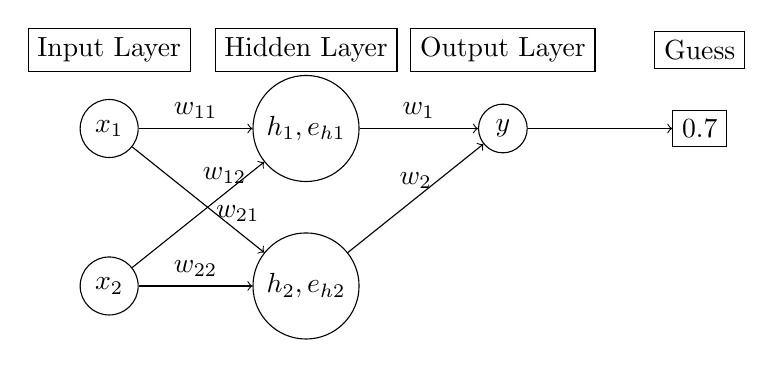
\begin{tikzpicture}
            \node[draw] (A) at (0, 0) {Input Layer};
            \node[draw] (B) at (\dist, 0) {Hidden Layer};
            \node[draw] (C) at (2*\dist, 0) {Output Layer};
            \node[draw] (D) at (3*\dist, 0) {Guess};
            
            \node[draw, circle] (iln1) at (0, -1) {\(x_1\)};
            \node[draw, circle] (iln2) at (0, -3) {\(x_2\)};

            \node[draw, circle] (hln1) at (\dist, -1) {\(h_1, e_{h1}\)};
            \node[draw, circle] (hln2) at (\dist, -3) {\(h_2, e_{h2}\)};

            \node[draw, circle] (oln1) at (2*\dist, -1) {\(y\)};
            \node[draw] (guess) at (3*\dist, -1) {0.7};

            \draw[->] (iln1) -- node[above] {\(w_{11}\)} (hln1);
            \draw[->] (iln1) -- node[pos=0.8, above] {\(w_{21}\)} (hln2);
            \draw[->] (iln2) -- node[pos=0.7, above] {\(w_{12}\)} (hln1);
            \draw[->] (iln2) -- node[above] {\(w_{22}\)} (hln2);

            \draw[->] (hln1) -- node[above] {\(w_1\)} (oln1);
            \draw[->] (hln2) -- node[above] {\(w_2\)} (oln1);
            \draw[->] (oln1) -- (guess);


        \end{tikzpicture}
    \end{center}
    known answer = 1
    \\
    error = \(1-0.7=0.3\) 
    \\
    We can use the error to nudge a weight, \(w_n\). But, how do we know what weight we need to nudge?
    \\
    \\
    \(e_{h1} = ???\)
    \\
    \(e_{h2} = ???\)
    \\
    Knowing these two errors, we can then adjust the weights between the hidden layer and input layer. But how do we find those errors?

\section{Breaking It Down}
    \begin{center}
        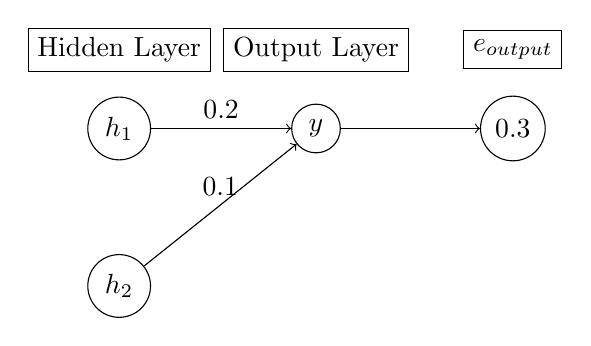
\begin{tikzpicture}
            \node[draw] (A) at (0, 0) {Hidden Layer};
            \node[draw] (B) at (\dist, 0) {Output Layer};
            \node[draw] (C) at (2*\dist, 0) {\(e_{output}\)};

            \node[draw, circle] (w1) at (0, -1) {\(h_1\)};
            \node[draw, circle] (w2) at (0, -3) {\(h_2\)};
            \node[draw, circle] (y) at (\dist, -1) {\(y\)};
            \node[draw, circle] (e) at (2*\dist, -1) {\(0.3\)};

            \draw[->] (w1) -- node[above] {\(0.2\)} (y);
            \draw[->] (w2) -- node[above] {\(0.1\)} (y);
            \draw[->] (y) -- node[above] {} (e);
        \end{tikzpicture}
    \end{center}

    \begin{equation}
        e_{h1} = \frac{w_1}{w_1+w_2} e_{output}
    \end{equation}
    \begin{equation}
        e_{h2} = \frac{w_2}{w_1+w_2} e_{output}
    \end{equation}

    \subsection{Adding Another Output}
    \begin{center}
        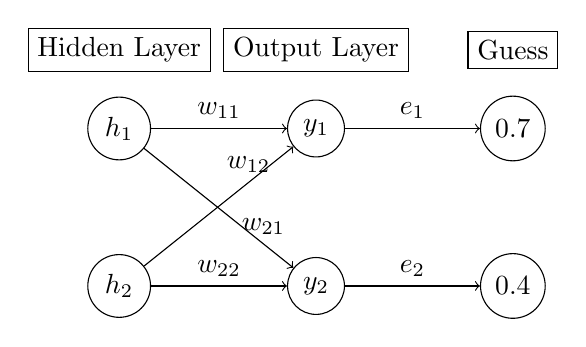
\begin{tikzpicture}
            \node[draw] (A) at (0, 0) {Hidden Layer};
            \node[draw] (B) at (\dist, 0) {Output Layer};
            \node[draw] (C) at (2*\dist, 0) {Guess};

            \node[draw, circle] (w1) at (0, -1) {\(h_1\)};
            \node[draw, circle] (w2) at (0, -3) {\(h_2\)};
            \node[draw, circle] (y1) at (\dist, -1) {\(y_1\)};
            \node[draw, circle] (y2) at (\dist, -3) {\(y_2\)};

            \node[draw, circle] (e1) at (2*\dist, -1) {\(0.7\)};
            \node[draw, circle] (e2) at (2*\dist, -3) {\(0.4\)};

            \draw[->] (w1) -- node[above] {\(w_{11}\)} (y1);
            \draw[->] (w2) -- node[pos=0.7, above] {\(w_{12}\)} (y1);
            \draw[->] (w1) -- node[pos=0.8, above] {\(w_{21}\)} (y2);
            \draw[->] (w2) -- node[above] {\(w_{22}\)} (y2);

            \draw[->] (y1) -- node[above] {\(e_1\)} (e1);
            \draw[->] (y2) -- node[above] {\(e_2\)} (e2);
        \end{tikzpicture}
    \end{center}

    \begin{equation}
        e_{h1} = \frac{w_{11}}{w_{11}+w_{12}} e_{1} + \frac{w_{21}}{w_{21}+w_{22}} e_{2}
    \end{equation}

    \begin{equation}
        e_{h2} = \frac{w_{12}}{w_{12}+w_{11}} e_{1} + \frac{w_{22}}{w_{22}+w_{21}} e_{2}
    \end{equation}

    We don't necessarily need the bottom part of the fraction because it ends up all canceling out. So now we can write\dots
    
    \begin{equation}
        e_{h1} = w_{11}e_1+w_{21}e_2
    \end{equation}

    \begin{equation}
        e_{h2} = w_{12}e_1+w_{22}e_2
    \end{equation}

    Now putting it into matrix terms\dots

    \begin{equation}
        \begin{bmatrix}
            e_{h1} \\
            e_{h2}
        \end{bmatrix}
        =
        \begin{bmatrix}
            w_{11} & w_{21} \\
            w_{12} & w_{22}
        \end{bmatrix}
        \begin{bmatrix}
            e_1 \\
            e_2
        \end{bmatrix}
    \end{equation}

    Oh and by the way\dots

    \begin{equation}
        w_{l} = 
        \begin{bmatrix}
            w_{11} & w_{12} & \dots \\
            w_{21} & w_{22} & \dots \\
            \dots & \dots & \dots
        \end{bmatrix}^{T}
    \end{equation}

    \begin{equation}
        w_{l}^{T} = 
        \begin{bmatrix}
            w_{11} & w_{12} & \dots \\
            w_{21} & w_{22} & \dots \\
            \dots & \dots & \dots
        \end{bmatrix}^{T}
        = 
        \begin{bmatrix}
            w_{11} & w_{21} & \dots \\
            w_{12} & w_{22} & \dots \\
            \dots & \dots & \dots
        \end{bmatrix}
    \end{equation}

    Which is the same as the first matrix in equation 7.

    \subsubsection{Example With XOR Gate}
    
    \def\disttwo{3}
    \begin{tikzpicture}
        \node[draw] (IL) at (0, 0) {Input Layer};
        \node[draw] (HL1) at (\disttwo, 0) {Hidden Layer 1};
        \node[draw] (HL2) at (2*\disttwo, 0) {Hidden Layer 2};
        \node[draw] (IL) at (3*\disttwo, 0) {Output Layer};

        \node[draw, circle] (IN1) at (0, -1) {};
        \node[draw, circle] (IN2) at (0, -3) {};

        \node[draw, circle] (HL1N1) at (\disttwo, -1) {};
        \node[draw, circle] (HL1N2) at (\disttwo, -3) {};

        \node[draw, circle] (HL2N1) at (2*\disttwo, -1) {};
        \node[draw, circle] (HL2N2) at (2*\disttwo, -3) {};

        \node[draw, circle] (OP1) at (3*\disttwo, -1) {};

        \draw[->] (IN1) -- node[above] {\(w_{L1_{11}}\)} (HL1N1);
        \draw[->] (IN1) -- node[pos=0.8, above] {\(w_{L1_{21}}\)} (HL1N2);
        \draw[->] (IN2) -- node[pos=0.7, above] {\(w_{L1_{12}}\)} (HL1N1);
        \draw[->] (IN2) -- node[above] {\(w_{L1_{22}}\)} (HL1N2);

        \draw[->] (HL1N1) -- node[above] {\(w_{L2_{11}}\)} (HL2N1);
        \draw[->] (HL1N1) -- node[pos=0.8, above] {\(w_{L2_{21}}\)} (HL2N2);
        \draw[->] (HL1N2) -- node[pos=0.7, above] {\(w_{L2_{12}}\)} (HL2N1);
        \draw[->] (HL1N2) -- node[above] {\(w_{L2_{22}}\)} (HL2N2);

        \draw[->] (HL2N1) -- node[above] {\(w_{L3_{11}}\)} (OP1);
        \draw[->] (HL2N2) -- node[above] {\(w_{L3_{12}}\)} (OP1);

    \end{tikzpicture}

    Calulating output error and hidden errors in backpropigation, where \(e_{o}\) is the output error, \(i\) reprsents the ith sample,
    \(y\) reprsents the expected value, and \(\hat{y}\) reprsents the actual value.
    \begin{equation}
        e_{o_{i}} = y_i - \hat{y}_i
    \end{equation}

    \begin{equation}
        e_{L2} = 
        \begin{bmatrix}
            e_{o_i}
        \end{bmatrix}
        \begin{bmatrix}
            w_{L3_{11}} \\
            w_{L3_{12}}
        \end{bmatrix}
    \end{equation}

    \section{Adjusting Weights}
    \subsection{Gradient Descent}
    \begin{equation}
        y = mx+b
    \end{equation}

    \begin{equation}
        \Delta m = learningRate * x * error_j
    \end{equation}

    \begin{equation}
        \Delta b = learningRate * error_j
    \end{equation}

    How do we apply these equations to multivariable equations? In our case, we have\dots

    \begin{equation}
        y = \sigma (wI + b)
    \end{equation}

    \begin{equation}
        \sigma^{'}(x) = \sigma(x) + (1 - \sigma(x))
    \end{equation}

    \begin{equation}
        \Delta w^{HO}_{ij} = \alpha E_{L} (Output(1 - Output)) H^T 
    \end{equation}

    \begin{equation}
        \Delta w^{IH}_{ij} = \alpha H_e (H(1 - H)) I^T
    \end{equation}

    Where \(i\) and \(j\) is the current weight in the matrix, and \(HO\) 
    sisgnifies the hidden layer to the output layer. \(\alpha\) sisgnifies the 
    learning rate, and \(E_L\) is the error vector for the layer. \(H\) is what is 
    coming out of a hidden layer.


\end{document}